\chapter{What is Context?}

While trying to define context for the photo application domain, we found the existing definitions lacking one aspect or another. This is due to their object-centric view of context. In contrast, for an application with scope as broad as photo tagging, this chapter draws emphasis to a relation-centric view of context, and differentiate it from previous object centric definitions. Later, these properties of context are used to specify what objects and relationships are most relevant to the tagging problem.
	
\begin{figure}[h]
\centering
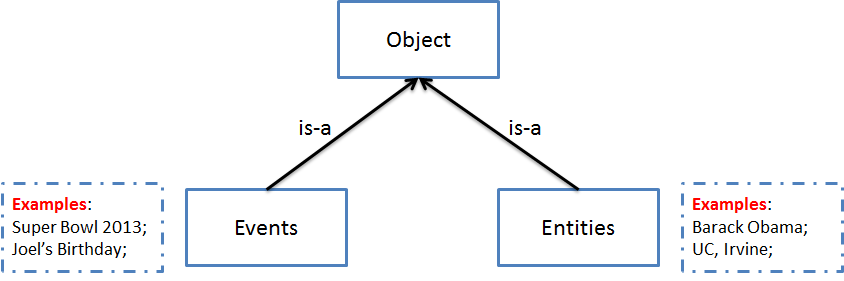
\includegraphics[width=0.6\textwidth]{media/chapter1/terminology.png}
\caption{Objects, Events and Entities.}
\label{fig:terminology}
\end{figure}

Before looking at the different views on context, its advisable to distinguish between `objects' and `entities'. We use the word `Object' to collectively refer to events and entities. The term `object' has been used in literature to refer to things which have no temporal properties. But, in our discussion, an `object' could imply an event which exhibits temporal properties. An entity includes persons, places in the world, for example `Starbucks, UC Irvine', `The Eiffel Tower, Paris, France', or organizations, for example `Google Inc', `Royal Society of London'. Effectively, they are objects which do not need temporal descriptors. Events, on the other hand, are objects which rely on temporal attributes.

Our justification for the use of context in a personal face tagging application begins with the assumption: \textit{For a given user, the correctness of face tags for a photograph containing people she has never met is undefined}. This observation prepares us to understand what context is, and how contextual reasoning assists in tagging photos. The description of any problem domain requires a set of abstract data types, and a model of how these types are related to each other. We define contextual types as those which are semantically different from these data types, but can be directly or indirectly related to them via an extended model which encapsulates the original one. Contextual reasoning assists in the following two ways. \textbf{First}, contextual data restricts the number of people who might appear in the photographs. We can also argue that all the personal data of a user (her profile on Facebook, LinkedIn, email exchanges, phone call logs) provides a reasonable estimate of all these people who might appear in her photos. \textbf{Second}, by reasoning on abstractions in the contextual domain, we can infer conclusions on the original problem. We exploit this property to develop our algorithm in the later sections. Though context based search space pruning can be applied to a variety of recognition problems, we focus on tagging people in personal photos for concreteness, where, the image and person tag form the abstractions in the problem domain, and events and event based relations constitute the contextual domain. 

\section{Previous Definitons}

One of the earliest studies on context was done by Bill Schilit et al.\ in \cite{schilit1994context}. The focus in this study was how to build software in dynamic environments. The dynamics of the environments were largely due to people requiring different computational services at the different times, the modality of request (through a mobile device or through a workstation), and the environment of the device (are there cameras and projectors nearby if the task requires video conferencing?). This software-centric view of context highlights the importance of two things. One, context is always described with respect to an object. In this case it is the software which runs on processors distributed in a real world environment. Second, context is used to determine how this object interacts with events and entities near it? For example, Schilit uses the example that a workstation should automatically load his favorite text editor when he approaches it; and an rooster music sample must be played whenever fresh coffee is prepared. Both very different and precise interactions even though they might share common background (environment or participating entities). We would not expect a text editor to be shown when coffee is prepared, and the rooster music to be played when an employee walks to a workstation.

\begin{figure}[t]
\centering
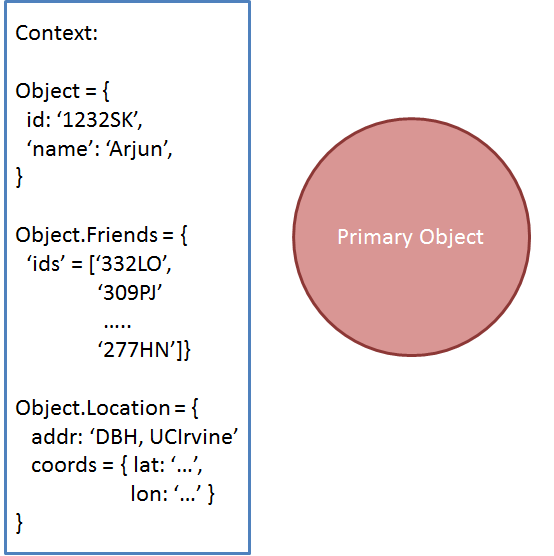
\includegraphics[width=0.5\textwidth]{media/chapter2/dey-def.png}
\caption{Information related to the situation of an Object.}
\label{fig:anind-def}
\end{figure}

In his seminal paper, Anind Dey \cite{dey2001understanding} describes context \textit{as any information that can be used to characterize the situation of an entity. An entity is a person, place or object that is considered relevant to the interaction between a user and an application, including the user and applications themselves}, as shown in figure \ref{fig:anind-def}. He proceeds to explain this definition with the example of an ``indoor mobile tour", arguing that there are there are two additional pieces of information which can be used: \textit{weather} and \textit{presence of other people}. if the user is present with his friends, they might visit sites that are of interest to everybody. There the presence of other people is important context. Because the tour is indoor, weather does not affect the application. It is true that the weather has no direct affect on the application but what about the following scenarios:

\begin{itemize}
\item Could we use the weather information to serve different drinks in the cafeteria to boost the experience of the visitors? On a cold day, placing the hot chocolate kiosk next to the entrance and the ice cream kiosk closer on a warmer day might boost some sales.
\item If the tour is similar to Alcatraz, where a ferry ride takes people to the island, and back from it, a storm brewing in the ocean could lead to disrputed ferry services. Should the application warn its users who are liesurely touring at this time? Or should they continue the tour at the same pace, miss the last ferry and spend the night at Alcatraz? After all, accommodation is not a problem.
\end{itemize}

They then proceed to define Context-Aware computing as follows: \textit{A system is context-aware if it uses context to provide relevant information and/or services to the user, where relevancy depends on the user's tasks}. But, we need to ask ourselves why a system which uses this ``additional information" should be considered a context-aware system? There are numerous systems which would simply consider these ``additional information" as regular inputs. What is different between a system which takes in these inputs as processes them as regular data, and one which processes them as context?

\begin{figure}[t]
\centering
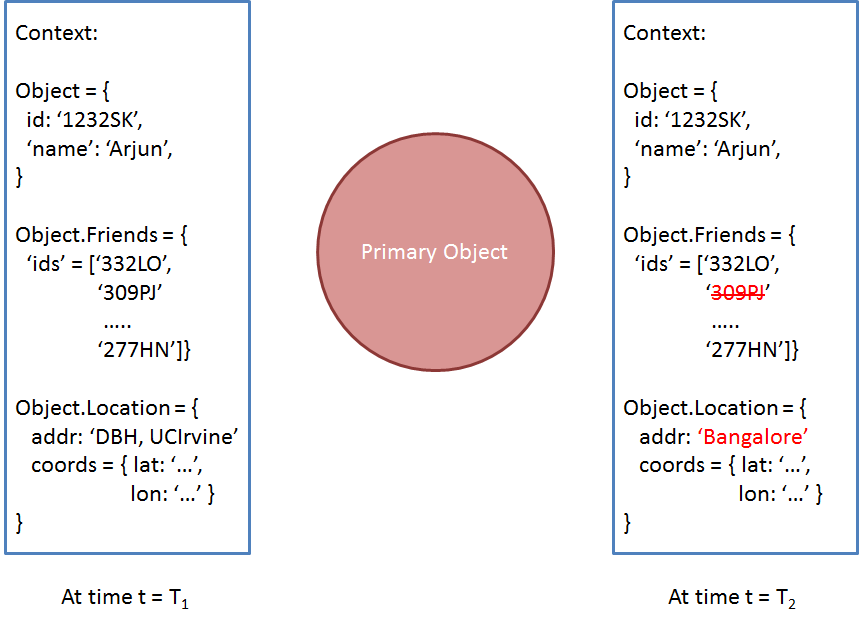
\includegraphics[width=0.75\textwidth]{media/chapter2/ka-obs.png}
\caption{Henricksen's observation about temporality of Context.}
\label{fig:karen-obs}
\end{figure}

Karen Henricksen et al.\ \cite{henricksen2002modeling} make the following interesting observation about context: Context information exhibits a range of temporal characteristics. Some context information can be static, for example the attributes of people using a system (for example, the sex of a person). But a large amount of information is dynamic. For example, the current geo position of a person or her social network, as shown in figure \ref{fig:karen-obs}. There is no straightforward way to obtain this dynamic information other than through sensors. But, such a approach tightly couples the application logic to the types of sensors used, and requires the system to convert the input data to usable representations. For example, the application requires explicit modules to convert GPS coordinates to readable addresses. The problem with such an approach is that there are many ad-hoc modules built to tackle the sensors, and therefore causing the context-awareness to be tied to a specific application.

More recently, Vaninha Vieira et al.\ \cite{vieira2011designing} uses a rule centric view of context to design their context sensitive system, Cemantika. Vaninha defines a contextual element as any piece of data or information which can be used to characterize an entity in an application domain, whereas the context of an interaction between an agent and an application is the set of instantiated contextual elements that are necessary to support the task at hand. Context awareness, for them, is to explicitly switch the task the system is executing under different conditions. For this they explictly model the \textit{context sources} which includes heterogenous and  external sources like sensors, user dialog interfaces and databases. Figure \ref{fig:va-def} shows various data sources providing context. Some data sources are preferred over others depending on certain conditions pre-defined in the system. This allows the various processes to operate independently of the type of sources. It should be noted that the use of ontologies is describing knowledge and context sources is becoming increasingly popular (more similar systems are described in chapter 3).

\begin{figure}[t]
\centering
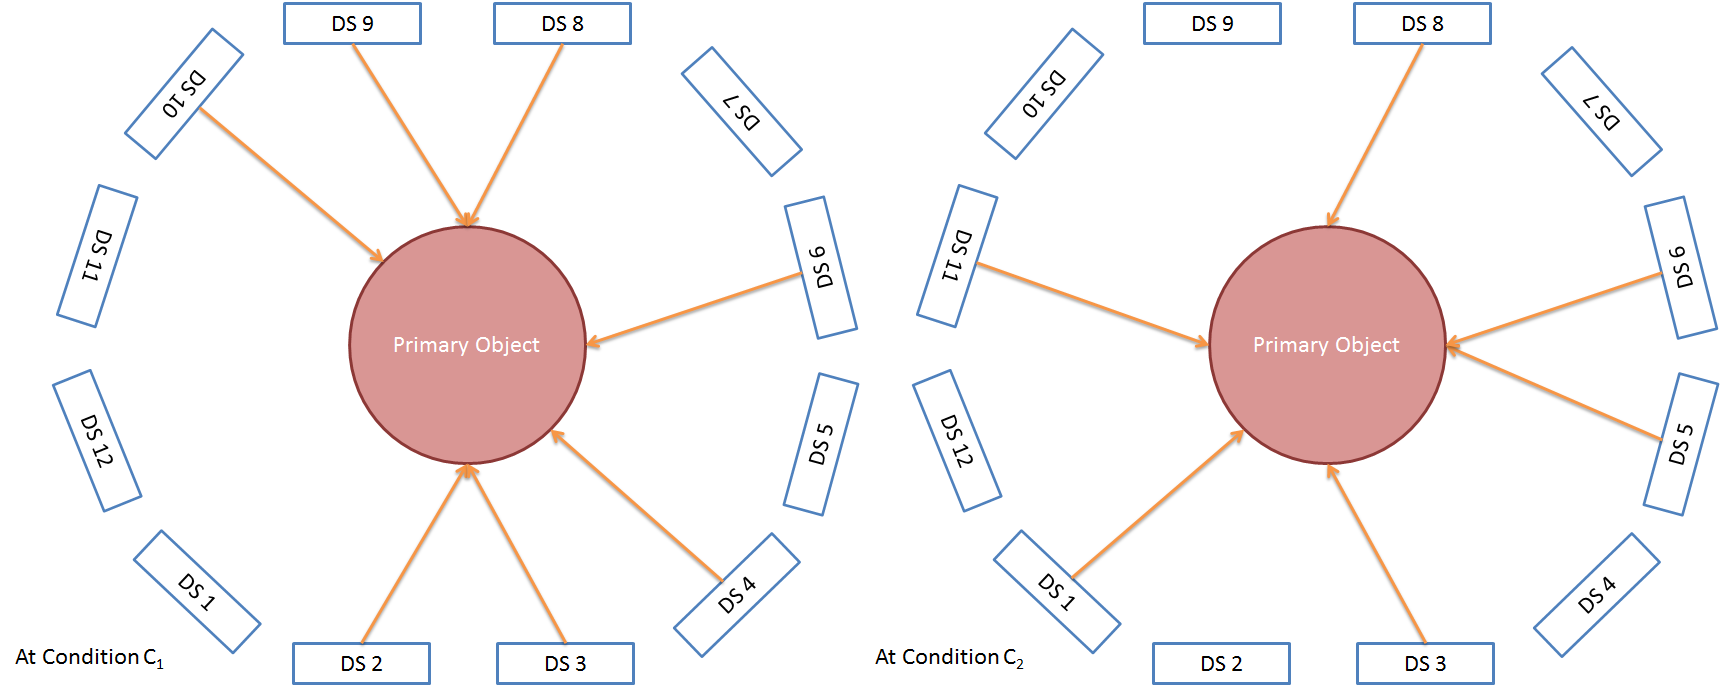
\includegraphics[width=\textwidth]{media/chapter2/va.png}
\caption{Modern context aware system obtain data from different sources.}
\label{fig:va-def}
\end{figure}

\section{Relation-Centric View of Context}

The common ground behind these definitions is their object centric view of context. Context is largely a set of objects that ``surrounds'' a primary object (whose context is in question). This view is insufficient while addressing applications which are very broad in scope, the photo tagging application for example, where users can take photos in very diverse environment, and a large number of sensors and sources of context exist. Specifically, it is non-trivial to identify which subset of available data qualifies to be relevant context for the given photo, and which is not. The two examples from chapter 1, are shown in figures \ref{fig:naaman-icmr} and \ref{fig:example-kasturi-show}. In order to tag the photo on the left, we exclusively used conference calendar information. Whereas, to tag the photo on the right, we used personal information. Our motivation in this chapter is to extend the above definitions of context to allow context aware systems to better extract relevant context from these various sources.

\begin{figure}[t]
\begin{minipage}[b]{0.48\linewidth}
\centering
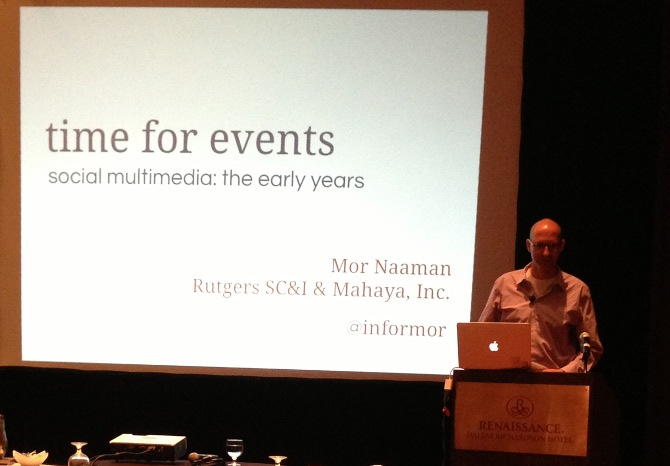
\includegraphics[width=\textwidth]{media/chapter2/naaman.jpg}
\caption{Mor Naaman at ICMR.}
\label{fig:naaman-icmr}
\end{minipage}
\hspace{0.5cm}
\begin{minipage}[b]{0.45\linewidth}
\centering
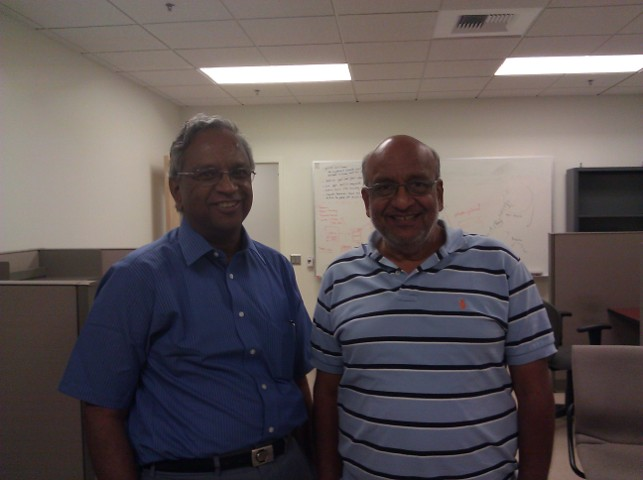
\includegraphics[width=\textwidth]{media/chapter1/kasturi-show.jpg}
\caption{Kasturi and Jain.}
\label{fig:example-kasturi-show}
\end{minipage}
\end{figure}

We define context of a given object at a particular time as \textbf{``the real world information which can be \uline{related to the object directly or indirectly} through a known set of relationships''}. Figure \ref{fig:cn-def} is an extension of \ref{fig:va-def} by making explicit the relations between various objects in the application ecosystem. Here, objects contained within two data sources can be related to each other. For example, an object in DS 9 can be related to another in DS 10 with the \texttt{related-to} edge. The primary object can be related to an object in DS 2 with an \texttt{occurs-at} relationship at time $t_1$. Whereas at time $t_2$, the relationship with DS 2 does not exist, but a new relationship \texttt{occurs-during} surfaces with DS 11.

\begin{figure}[t]
\centering
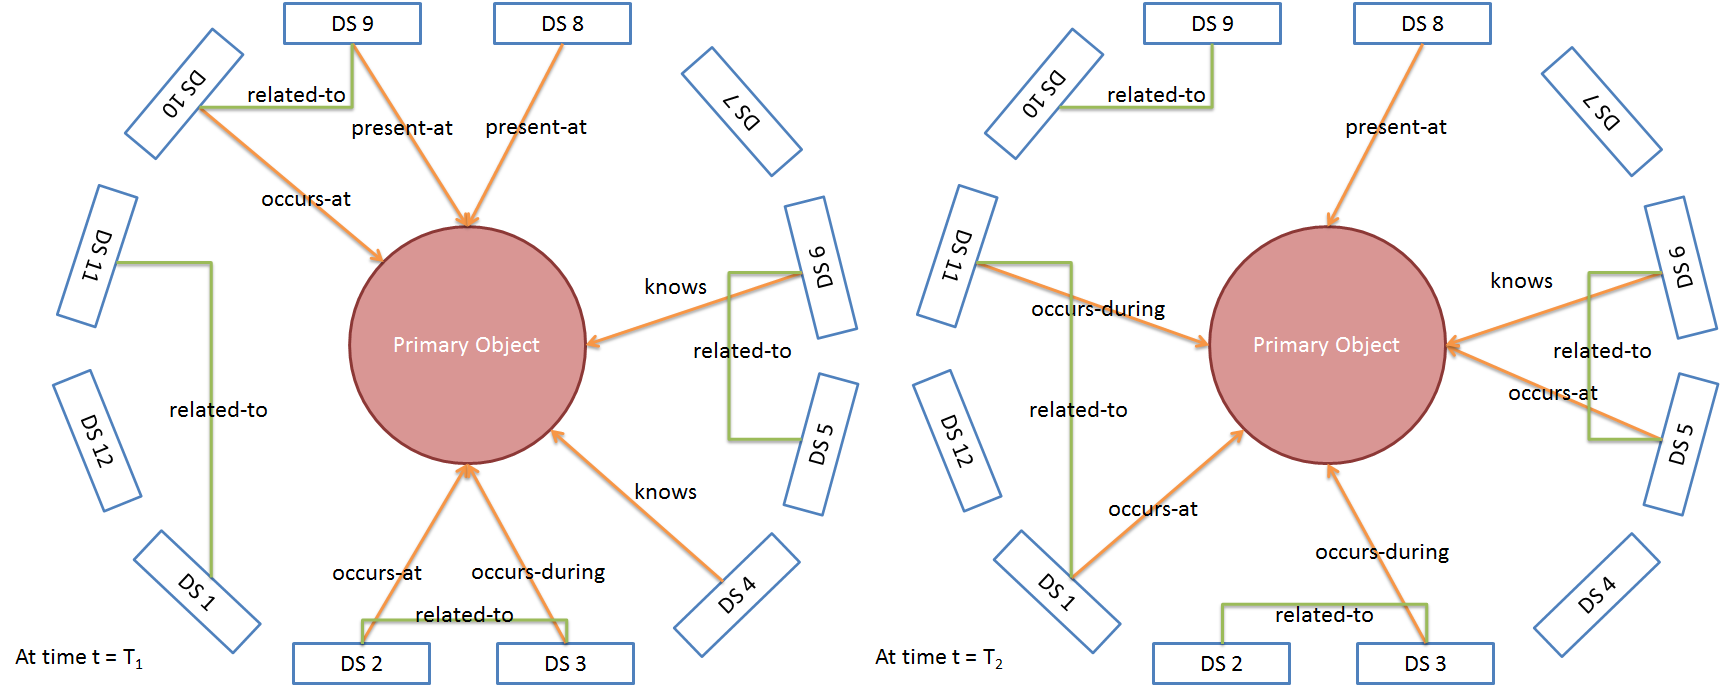
\includegraphics[width=\textwidth]{media/chapter2/cn.png}
\caption{Utilizing relations to define context for the primary object.}
\label{fig:cn-def}
\end{figure}

Relationships can be of different types. They can be simple labels like \texttt{friend-of} signifying a social relationship. Or they can more actionable like \texttt{located-at}, which relates a person to a particular location, and therefore causes a particular audio stream to play through the handheld device. This relation is not just a label, it imposes constraints on the properties of objects which it relates. Here, the spatial attributes of the the person and the exhibit must match if they are being related through a \texttt{located-at} attribute. In this dissertation, we will see that such relations, which impose such property constraints are critical in algorithmically determining which information is relevant context. Let us also assume that we have available to us the four types of data sources: event sources, place databases (like yelp.com), weather information sources and social networking information.

Using this relation centric view, we now look at how the examples from chapter 1 can be formulated in a systematic process to discover context. A system to discover context must establish a set of relationships its context objects can be connected with. For the two photos, we choose \textbf{participant-of}, which indicates that an entity is a participant in an event, and \textbf{subevent-of} which indicates that an event is occurring within another super-event. Thus, any entity can be related to other events through a \texttt{participant-of} edge, and events can be related to others events as well as entities through \texttt{subevent-of} and the \texttt{participant-of} edge respectively.

\begin{figure}[ht!]
\begin{minipage}[b]{0.48\linewidth}
\centering
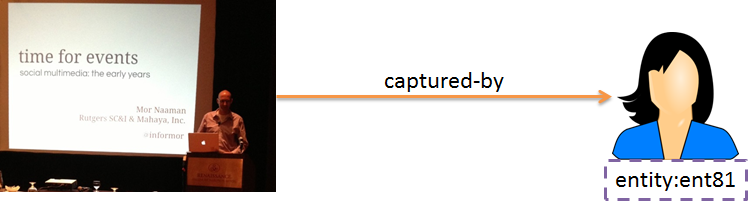
\includegraphics[width=\textwidth]{media/chapter2/naaman-1.png}
\caption{Primary objects.}
\label{fig:naaman-example-1}
\end{minipage}
\hspace{0.5cm}
\begin{minipage}[b]{0.45\linewidth}
\centering
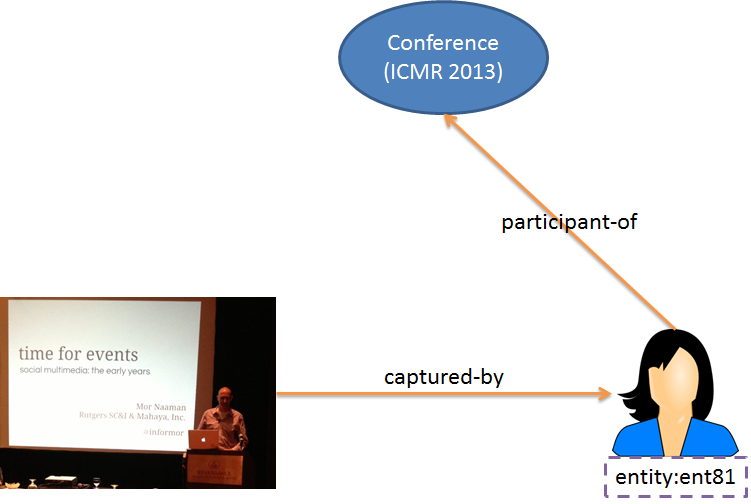
\includegraphics[width=\textwidth]{media/chapter2/naaman-2.png}
\caption{Associating \texttt{conference event} using the \texttt{participant-of} relation}
\label{fig:naaman-example-2}
\end{minipage}
\begin{minipage}[b]{0.48\linewidth}
\centering

\includegraphics[width=\textwidth]{media/chapter2/white.png}
\label{fig:naaman-example-x}
\end{minipage}
\hspace{0.5cm}
\begin{minipage}[b]{0.45\linewidth}
\centering

\includegraphics[width=\textwidth]{media/chapter2/white.png}
\label{fig:naaman-example-y}
\end{minipage}
\begin{minipage}[b]{0.48\linewidth}
\centering
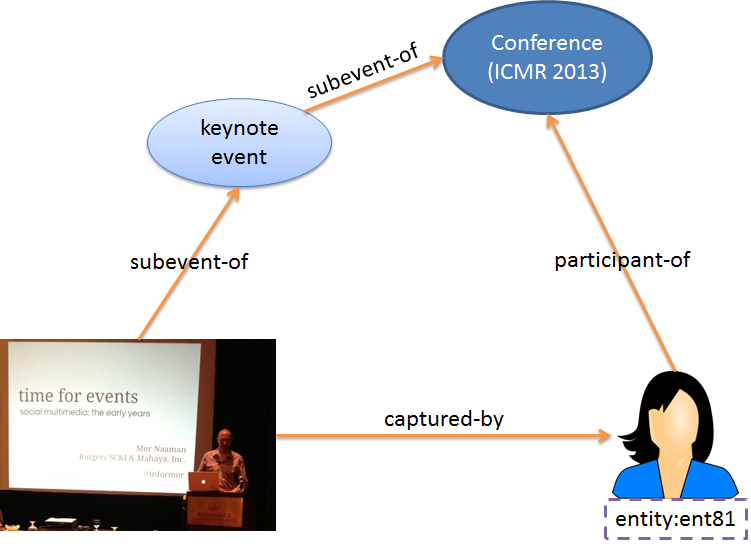
\includegraphics[width=\textwidth]{media/chapter2/naaman-3.png}
\caption{Associating the keynote event.}
\label{fig:naaman-example-3}
\end{minipage}
\hspace{0.5cm}
\begin{minipage}[b]{0.45\linewidth}
\centering
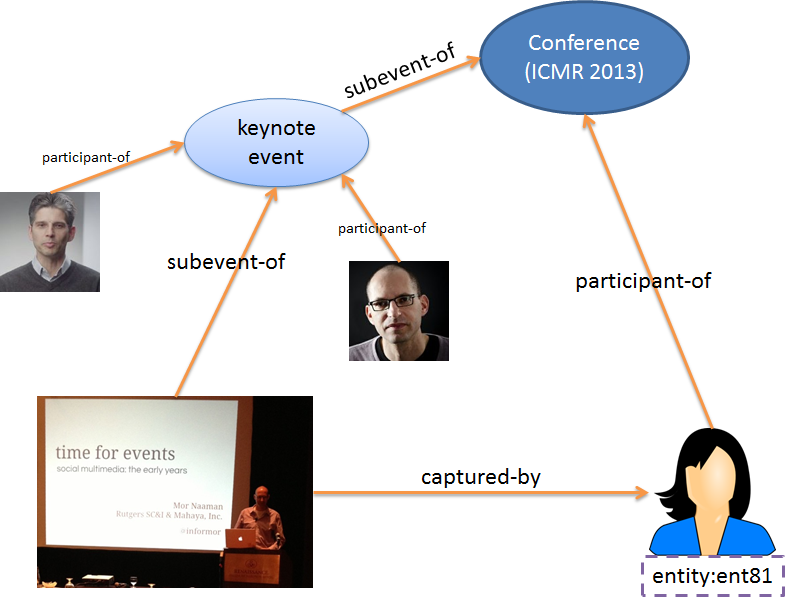
\includegraphics[width=\textwidth]{media/chapter2/naaman-4.png}
\caption{Associating the participants using the \texttt{participant-of} relation}
\label{fig:naaman-example-4}
\end{minipage}
\end{figure}

Figures \ref{fig:naaman-example-1} through \ref{fig:naaman-example-4} show how the two relationships can be used to gather context for the photo in figure \ref{fig:naaman-icmr}. Figure \ref{fig:naaman-example-1} shows the initial graph created using the \texttt{photo-capture-event} and the photographer, \texttt{entity:ent81}. Figure \ref{fig:naaman-example-2} shows the result of adding context by associating an event with \texttt{entity:ent81}. Given this new graph with three nodes, a context aware system can find more context by trying to find objects which can be related through the two edges. Since one of the nodes is a \texttt{conference} event, it proceeds to find events occurring within it, and adds the keynote event, which also happens to be the super-event of the \texttt{photo-capture-event}. The result is shown in figure \ref{fig:naaman-example-3}. Finally, the keynote event is extended with relations to associate subevents or participants. In this case, the only new context available are the participants of the keynote event. These two entities are associated with the event as shown in figure \ref{fig:naaman-example-4}. 

In the above example, given a graph containing primary objects, we grew it by relating objects from the real-world using a fixed set of relationships \{\texttt{participant-of}, \texttt{subevent-of}\}. Such a graph representing the primary objects, the context objects and their inter-relationships is a \textbf{context network}. Figure \ref{fig:context-network} shows one such context network for Mor Naaman's photo taken at ICMR 2013. A similar procedure can be invoked on the photo in figure \ref{fig:example-kasturi-show} to discover its context network.

Because of the type of relationships chosen, some information which was readily available (weather, place or social networking, for example) was not associated. But if we extend the relationship set to contain another relation \texttt{occurs-at}, then the place where the conference was held will be included in the context network. Similarly, the inclusion of a \texttt{knows} can relate entities with each other. If the social networking source reports that \texttt{entity:ent81} was a friend of Mor Naaman, an additional edge would be introduced between these nodes in the context network. Thus, relations are key in determining which objects are context and which are not, and how they are related to the primary objects.

\begin{figure}[h]
\centering
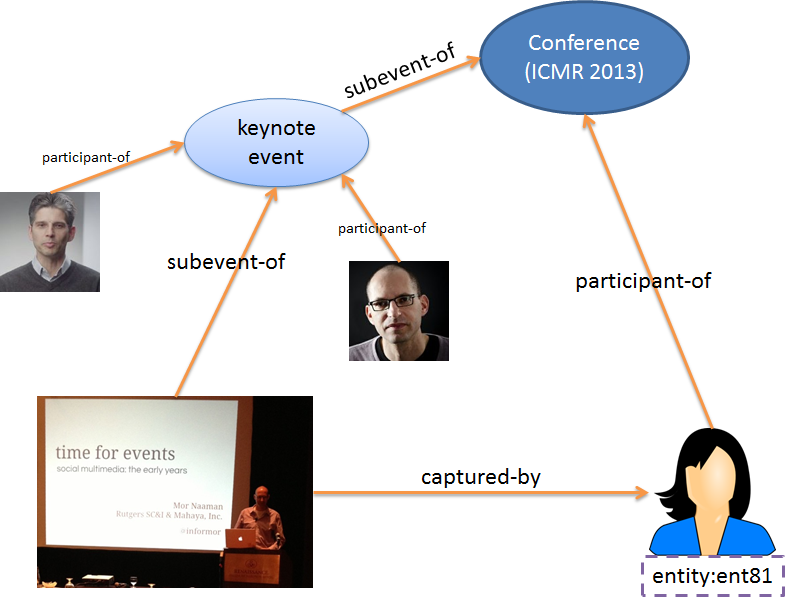
\includegraphics[width=0.75\textwidth]{media/chapter2/naaman-4.png}
\caption{Context Network for Mor Naaman's photo.}
\label{fig:context-network}
\end{figure}

It must be noted that asserting a relation-centric view of context is not discounting the importance of objects. Rather, it is a way of saying that relationships are atleast as important as objects are. Keeping this in mind, we will see what are the primitives required to model context for real-world problems in this section.

\section{Modeling Context for Real-world Problems}

There is no silver bullet to model context. Henricksen et al.\ \cite{henricksen2002modeling} model context using context graphs, and \cite{reignier2007context} provides a technique to construct petri nets for given context graphs to implement context-aware behavior. Although, these techniques work for specific domain (for example, \cite{reignier2007context} presents a domain of class presentations, and \cite{henricksen2002modeling} presents a case study in context-aware communications), creating context graphs to exist for each and every case which might occur in the real world is non-trivial. Also, with the rapidly changing relations in the real-world, it is not clear what are the good principles and practices to build scalable systems around context graphs.

If we are to represent context networks computationally, we first need to understand what are the basic building blocks of such a network. The following sections list these blocks, and present their properties which are essential in constructing such networks. These blocks are fairly generic, and can be utilized to model context for various application.

% NOTES
%The requirements must be split across different available tools (a more systems approach to modeling). Henrickson's CxG approach. Get rid of context awareness FULLY? 2.4.1, 2.4.2 part of 2.3; Dynamic linking is actually talking about source declaration. Write context awareness as a separate topic in the end of the chapter -- ``future work'', how the same tool now assist in multiple applications which involve photo taking.

\subsection{Object Types and Semantics}
Context is always specified with respect to a real world object. This primary object must be uniquely identifiable in the computational system, and must be an instance of one of the known classes. This object must have some real world attributes. For example, if the object is an event, then the interval during which it occurs, and location of occurence are two real world attributes. In the tour guide application, the visitor is one possible primary object whose context needs to determined. In the photo application, possible types of interest include the \texttt{photo-capture-event}, the \texttt{photographer}, various possible events which can occur in the world, people and places where photography can occur.

Different objects bring with them very specific semantics. While modeling objects as context, these semantics must be preserved. For example, an event object exists only for a fixed time interval. People can only be present at one place at one point in time. The \texttt{photographer} is a person, and therefore inherits the property of being at only one place at a time. In the later chapter, we will see that these semantic properties play a very important role in the context discovery algorithm.

\subsection{Relationships and Constraints}
Context is any event or entity which can be \textit{related} to the objects in a problem. Instead of finding objects which are of a specific type, and qualifying them as context, objects related to the problem variables through specific relationship types are to be considered context. These relationships can impose certain constraints on the objects which they relate. For example, the subevent relation requires that the super-event spatio-temporally contain the smaller event. Such constraints are very common in real-world relationships. Many examples can be seen in applications involving chemical reactions, where it is not sufficient to have just two reactants at the same time and place, but the reaction could demand very specific environmental factors (like temperature or pressure). The specification of the relationships for modeling context should permit the specification of these specific constraints.

\subsection{Temporal Semantics}
Modeling context requires the ability to express relationships which assert temporal constraints. For example, during a lunch break at a conference, there are no co-occuring session events; the workshops at a banquet is always the last event at a conference, which could be followed by one or more workshops. Temporal relations have been studied in literature \cite{allen1983maintaining, wolter2000spatio}, and can be reused for this purpose. Temporal relationships defined in Allen's Interval Algebra are shown in figure \ref{fig:allen}. Figure shows these relationships. In order to relate events with entities, we use the \texttt{occurs-during} relation defined in \cite{gupta2011managing}. For example, the event X is said to \texttt{occur-during} the interval $I$ iff X's temporal extent is equal-to $I$. Additional relations \texttt{occurs-sometime-during} and \texttt{occurs-during-n} are also defined in \cite{gupta2011managing}.

\begin{figure}[h]
\centering
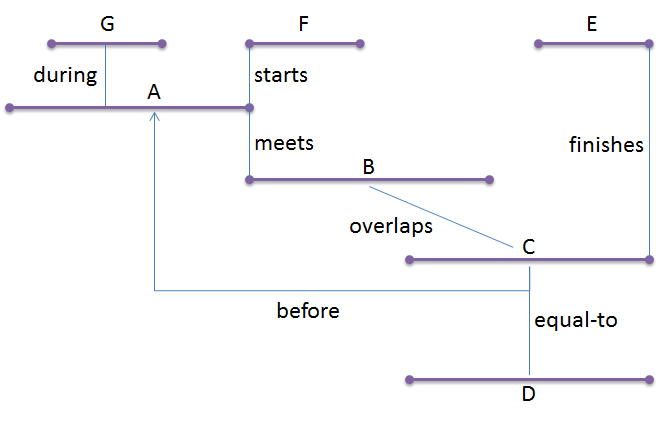
\includegraphics[width=0.75\textwidth]{media/chapter2/allen.png}
\caption{Intervals and their relations in Allen's Interval Algebra.}
\label{fig:allen}
\end{figure}

\subsection{Spatial Semantics}
Real-world events play an important role in context, and therefore, we need to pay special attention to the spatial relationships between entities and events. A large amount of literature is available on spatial representation and reasoning framework originally known as RCC-8. Some of its common relationships are shown in figure \ref{fig:rcc8}. The important relations in the figure are \texttt{disconnected} (B and D), \texttt{externally-connected} (B and C), \texttt{tangential-proper-part} (A and B), \texttt{contained-in} (E and D) and \texttt{partial-overlaps} (C and D). In order to represent spatial relations between events and entities, we use the \texttt{occurs-at} relation defined in \cite{gupta2011managing}. An event E is said to \texttt{occur-at} region $S$ if the spatial extent of E completely lies within $S$. Additional relations \texttt{occurs-somewhere-at} and \texttt{occurs-at-n} are also defined in \cite{gupta2011managing}.

\begin{figure}[h]
\centering
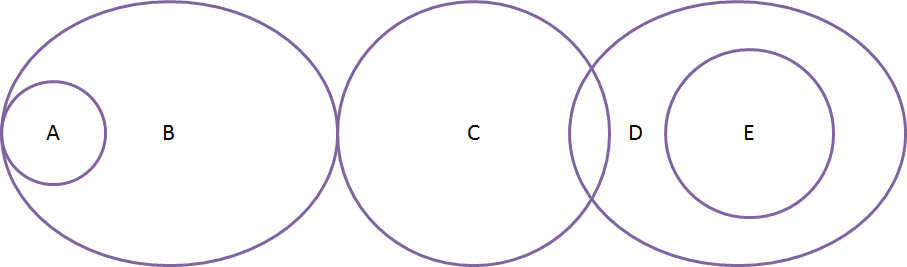
\includegraphics[width=0.75\textwidth]{media/chapter2/rcc8-combined.png}
\caption{Spatial regions which can be represented in the RCC-8 framework.}
\label{fig:rcc8}
\end{figure}

\subsection{Real-World Knowledge}
Modeling real world knowledge is critical in context based systems. This is in contrast with rule based systems, where a set of conditions are evaluated to trigger one or more actions. Examples of knowledge are: An academic conference has atleast one keynote talk; or Sodium reacts with atmospheric oxygen at room temperature; or water expands when it freezes. By explicitly modeling such networks of knowledge, we provide the opportunity to influence extraction of context from different sources. For example, if an object is associated with a keynote talk, data about the co-occuring conference is definitely going to be relevant context. Alternatively, if the system had associated a conference with the object, data about the keynote must be sought out. This `guiding light' trait of knowledge makes it an important pre-requisite in a context-aware system.

\subsection{Source Agnosticism}
Most context based techniques rely on sensors or data sources to gather context. Therefore, it must be imperative to separate the sources from how context is obtained. Context must be modelled irrespective of the nature of sources or their query abilities \cite{yerneni1999computing}. This provides the following advantage: context is now entirely defined in terms of objects, their possible inter-relationships and real world knowledge decides how objects are related to each other, irrespective of what data actually can be obtained. Second, with the growing number of data sources, personal and public sensors, this allows system engineers to plug-and-play different sources with ease, without disturbing the model. 

This design requirement also brings a problem. How does context-aware system know what data sources are at its disposal, and how does it interact with them? The short answer to this question is to utilize data integration technology \cite{doan2005semantic, halevy2001answering, lenzerini2002data}. Data integration techniques provide a uniform query interface to a multitude of autonomous data sources, irrespective of their native query capabilities or data storage formats. This might not be most ideal in the long run as these technologies were built to support RDBMS-like analytics operations, and we might benefit by adding more ``context operations" into the integration layers, thereby allowing more fruitful grounds for query otpimization. But for our current needs, it is advisable to re-use the ideas presented in these techniques to realize a fully working context-based system. The later chapters will describe in detail the data integration framework used to obtain data for the photo application.

\section{Context for Personal Photos}
The types used in the contextual domain, but not limited to, are the following:

\begin{itemize}
\item \textbf{Event Objects}: includes description of events like conferences, parties, trips or weddings, and their structure (for example, what kind of sessions, talks and keynotes are occurring within a particular conference).
\item \textbf{Entity Objects}: information about a user's social graph, people whom she corresponds with using email and other messaging services.
\item \textbf{Geographical Objects}: various tools like Facebook Places, Google Latitude or Foursquare provide information about where people are at a given time.
\end{itemize}

The important relations which dealing with such data are:

\begin{itemize}
\item \textbf{Subevent Relation}: If two events occur such that, one spatio-temporally contains the other, we say that it is the subevent of the one with larger spatio-temporal span. For example, a talk event is a subevent of the conference during which it happens.
\item \textbf{Participation Relation}: If an entity is participating in an event, s/he is said to be a participant-of that event. Note that this relation constraints the spatio-temporal boundary where the entity could be present during the interval of the event.
\item \textbf{Social Relation (knows)}: Social relations relate people who are acquainted with each other. This is used to model social networking information obtained from sources like Facebook or Email.
\item \textbf{Spatio-Temporal Relations}: Events occur in specific time intervals, and at some location. We use the relations occurs-at and occurs-during to model these properties. More details are provided in the next chapter.
\end{itemize}

\begin{figure}[h]
\centering
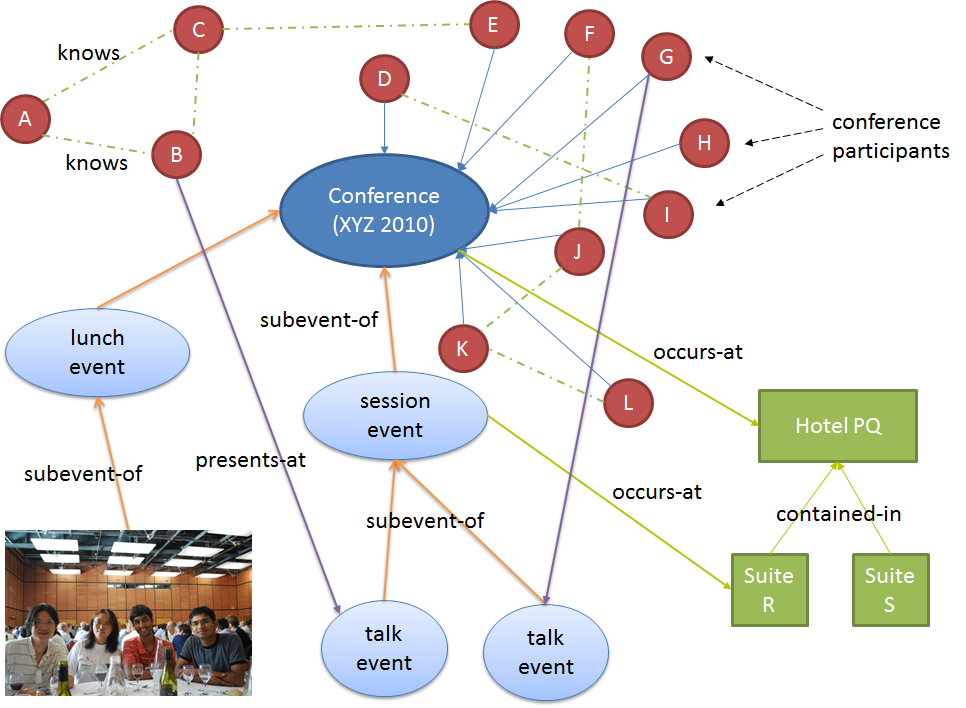
\includegraphics[width=0.85\textwidth]{media/chapter2/context-network-large.png}
\caption{A Context Network representing real world events, entities and their respective relationships.}
\label{fig:context-network-large}
\end{figure}

The above classes of contextual data can be obtained from a variety of data sources. Examples of data sources range from mobile phone call logs and email conversations to Facebook messages to a listing of public events at upcoming.com. We classify sources into the following types:

\begin{itemize}
\item \textbf{Metadata}: \textbf{TBD}
\item \textbf{Personal Data Sources}: include all sources which provide details about the particular user whose photo is to be tagged. Some common examples of personal data sources include Google Calendar, Email and Facebook profile and social graph.
\item \textbf{Social Data Sources}: include all sources which provide contextual information about a user's friends and colleagues. For example, LinkedIn, Facebook and DBLP are some of the commonly used websites with different types of social graphs.
\item \textbf{Public Data Sources}: include all sources which provide information about public organizations (like restaurants, points of interest or football stadiums) or about public events (like fairs, concerts or sports games).
\end{itemize}

\begin{figure}[h]
\centering
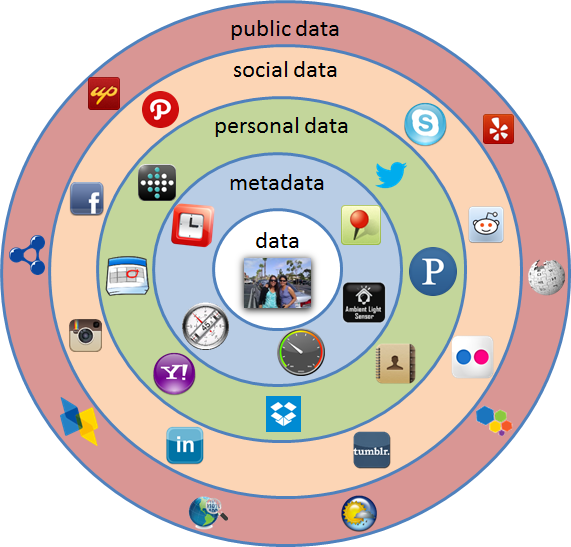
\includegraphics[width=0.85\textwidth]{media/chapter2/personal-social-public-data-sources.png}
\caption{Sources containing personal, social and public context for a given photo.}
\label{fig:personal-social-public-sources}
\end{figure}


Social and public data sources are enormous in size, containing information about billions of events and entities. Trying to use them directly will lead to scalability problems faced by face recognition and verification techniques. But, by using personal data, we can discover which parts of social and public sources are more relevant. For example, if a photo was taken at San Francisco, CA (where the user lives), his family in China is less relevant. Thus, the role of personal information is twofold. \textbf{Firstly}, it provides contextual information regarding the photo. \textbf{Secondly}, it acts as a bridge to connect to social and public data sources to discover interesting people connected to the user who might be present in the event and therefore, the photo.

At this point we should revisit the \textbf{temporal relevance} property of a data source. Given a stream of photos taken during a time interval, the source which contributed interesting context for a photo might not be equally useful for the one appearing next. This is because sources tend to focus on a specific set of event types or relationship types, and the two photos might be captured in different events or contains persons with whom the user maintains relations through different sources. For example, two photos taken at a conference might contain a user's friends in the first, but with advisers of these friends in the next. The friends might interact with the user through a social network, but their advisers might not. By using a source like DBLP, the relations between the adviser and friends can be discovered. We say that the temporal relevance of these context sources is \textbf{\textit{low}}. This requirement will play an important role in the design of our framework, as now, sources are not hardwired to photo, but instead need to be discovered gradually.

In short, the problem to be tackled is to construct context networks similar to the one shown in figure \ref{fig:context-network-large} using metadata, personal, social and public sources as shown in figure \ref{fig:personal-social-public-sources}. This problem will be resolved using our context discovery algorithm, presented in chapter 4. The next chapter, will present a short survey of various techniques relevant to our problem, and highlight the important ideas which helped develop the algorithms presented in this dissertation.